\documentclass{beamer}
\usepackage{times, amsfonts, amsmath, amssymb, latexsym, setspace, graphicx}
\usepackage{caption,subcaption}

\title{Visualizing Data }
\author{Guenther Walther}

\begin{document}
\frame{\titlepage}

\begin{frame}
Why does visualization matter?\\
\begin{itemize}
\item Large size of data makes it necessary to provide summaries.
\item People prefer to look at figures rather than numbers.
\end{itemize}
\bigskip

The two most important functions of visualizations are:\\
\begin{enumerate}
\item Communicate information
\item Support reasoning about data
\end{enumerate}
\end{frame}

\begin{frame}
\frametitle{Communicate information}
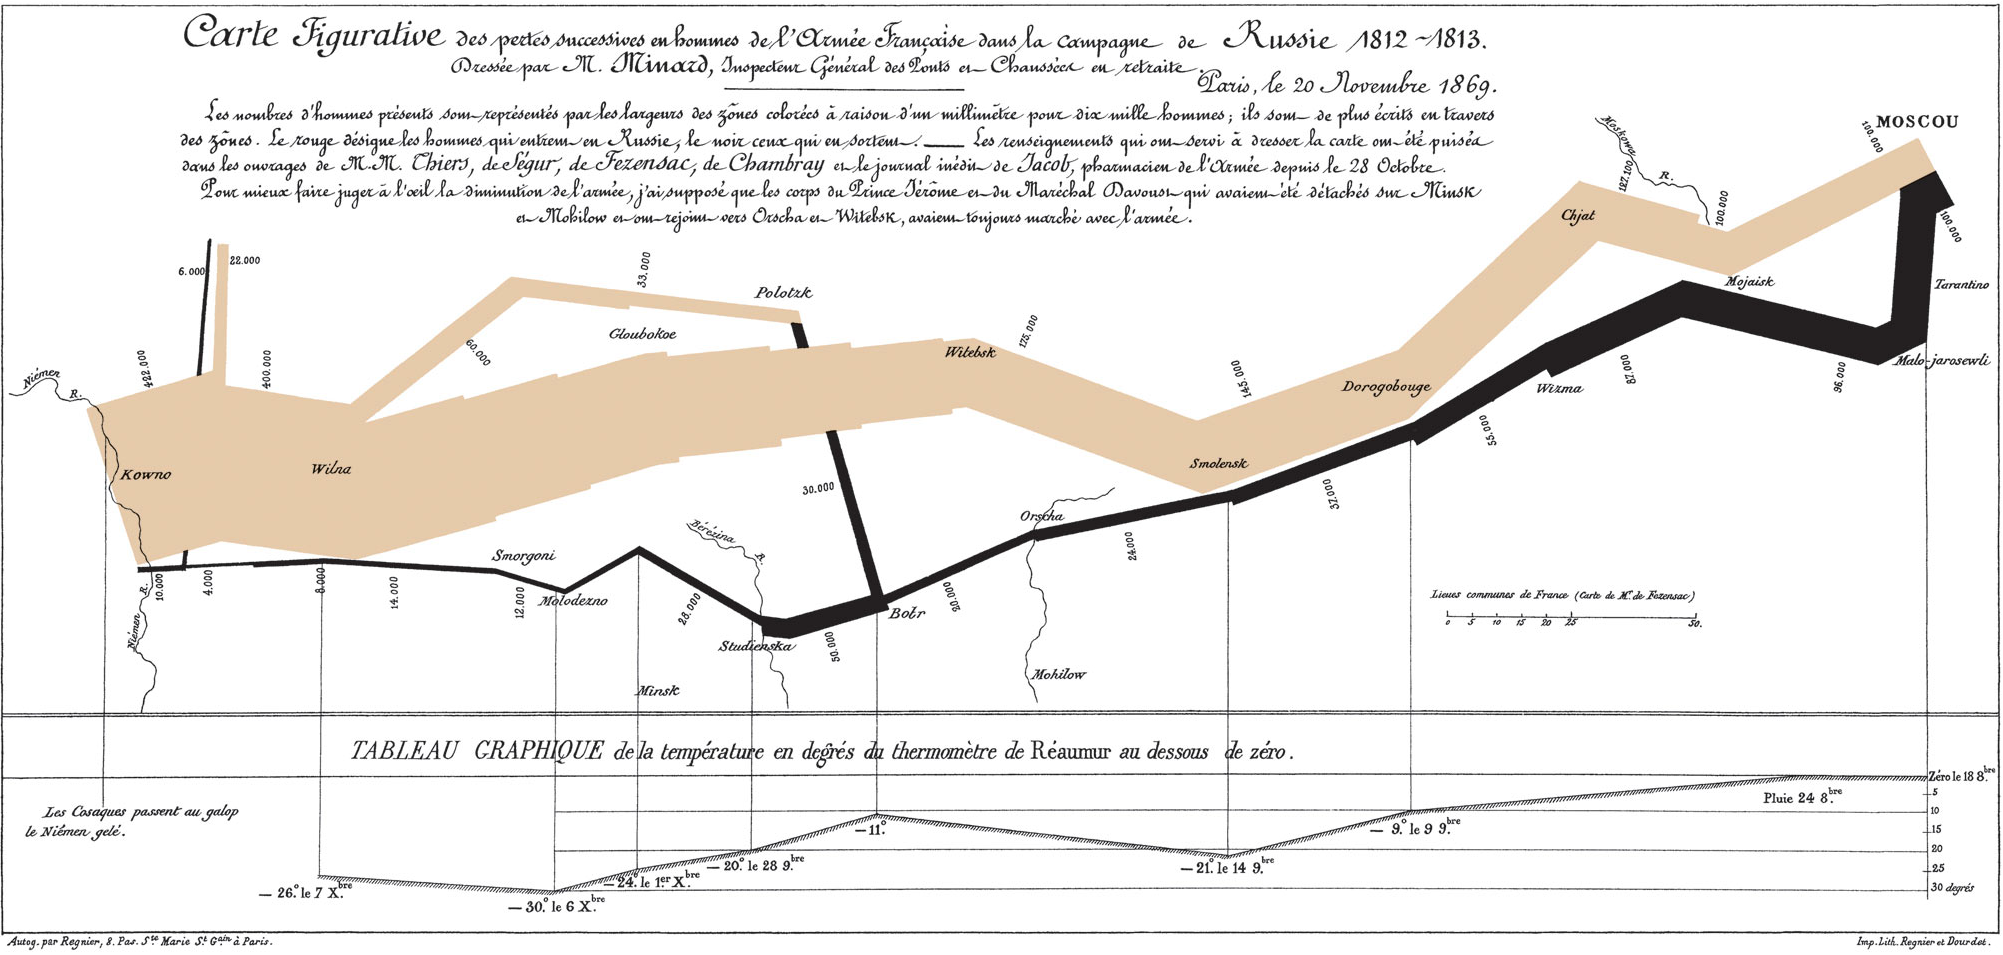
\includegraphics[width=\linewidth]{Minard}
\end{frame}

\begin{frame}
\frametitle{Support reasoning about about data}
On January 28, 1986, the space shuttle Challenger exploded
because two rubber O-rings leaked due to the very cold temperatures
at launch day. 
\medskip

This potential problem was discussed the day before the launch:
Engineers opposed launching based on data from previous launches, 
and provided 13 charts to NASA
to support their case. However, it is difficult to assess
the relationship between temperature and O-ring damage based on these
charts.
\end{frame}

\begin{frame}
\frametitle{Support reasoning about about data}
A visual display of the data from the investigation after the launch.
The poor design and use of chart junk makes it difficult to assess the
relationship between temperature and O-ring damage.

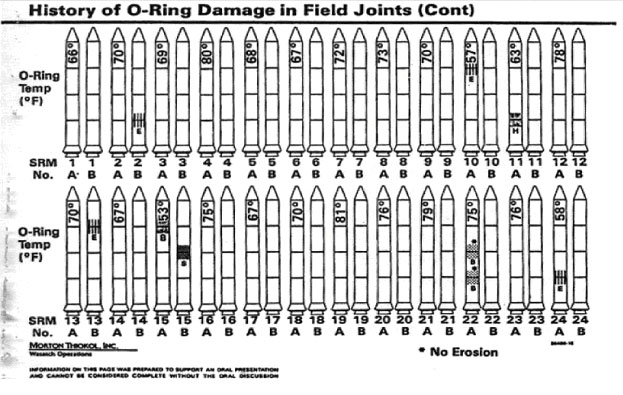
\includegraphics[width=\linewidth]{ChallengerBad}
\end{frame}

\begin{frame}
\frametitle{Support reasoning about about data}
A simple but pertinent display supports reasoning about the data. (from Tufte)
\medskip

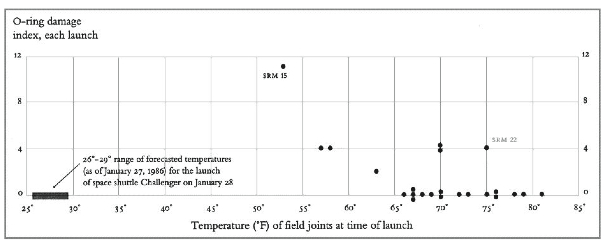
\includegraphics[width=\linewidth]{ChallengerGood}
\end{frame}

\begin{frame}
\frametitle{Elementary ways to display univariate data}

\begin{columns}[T]
\begin{column}{0.5\linewidth}
{\bf Pie chart}: the size of the angle\\
is proportional to the relative frequency\\
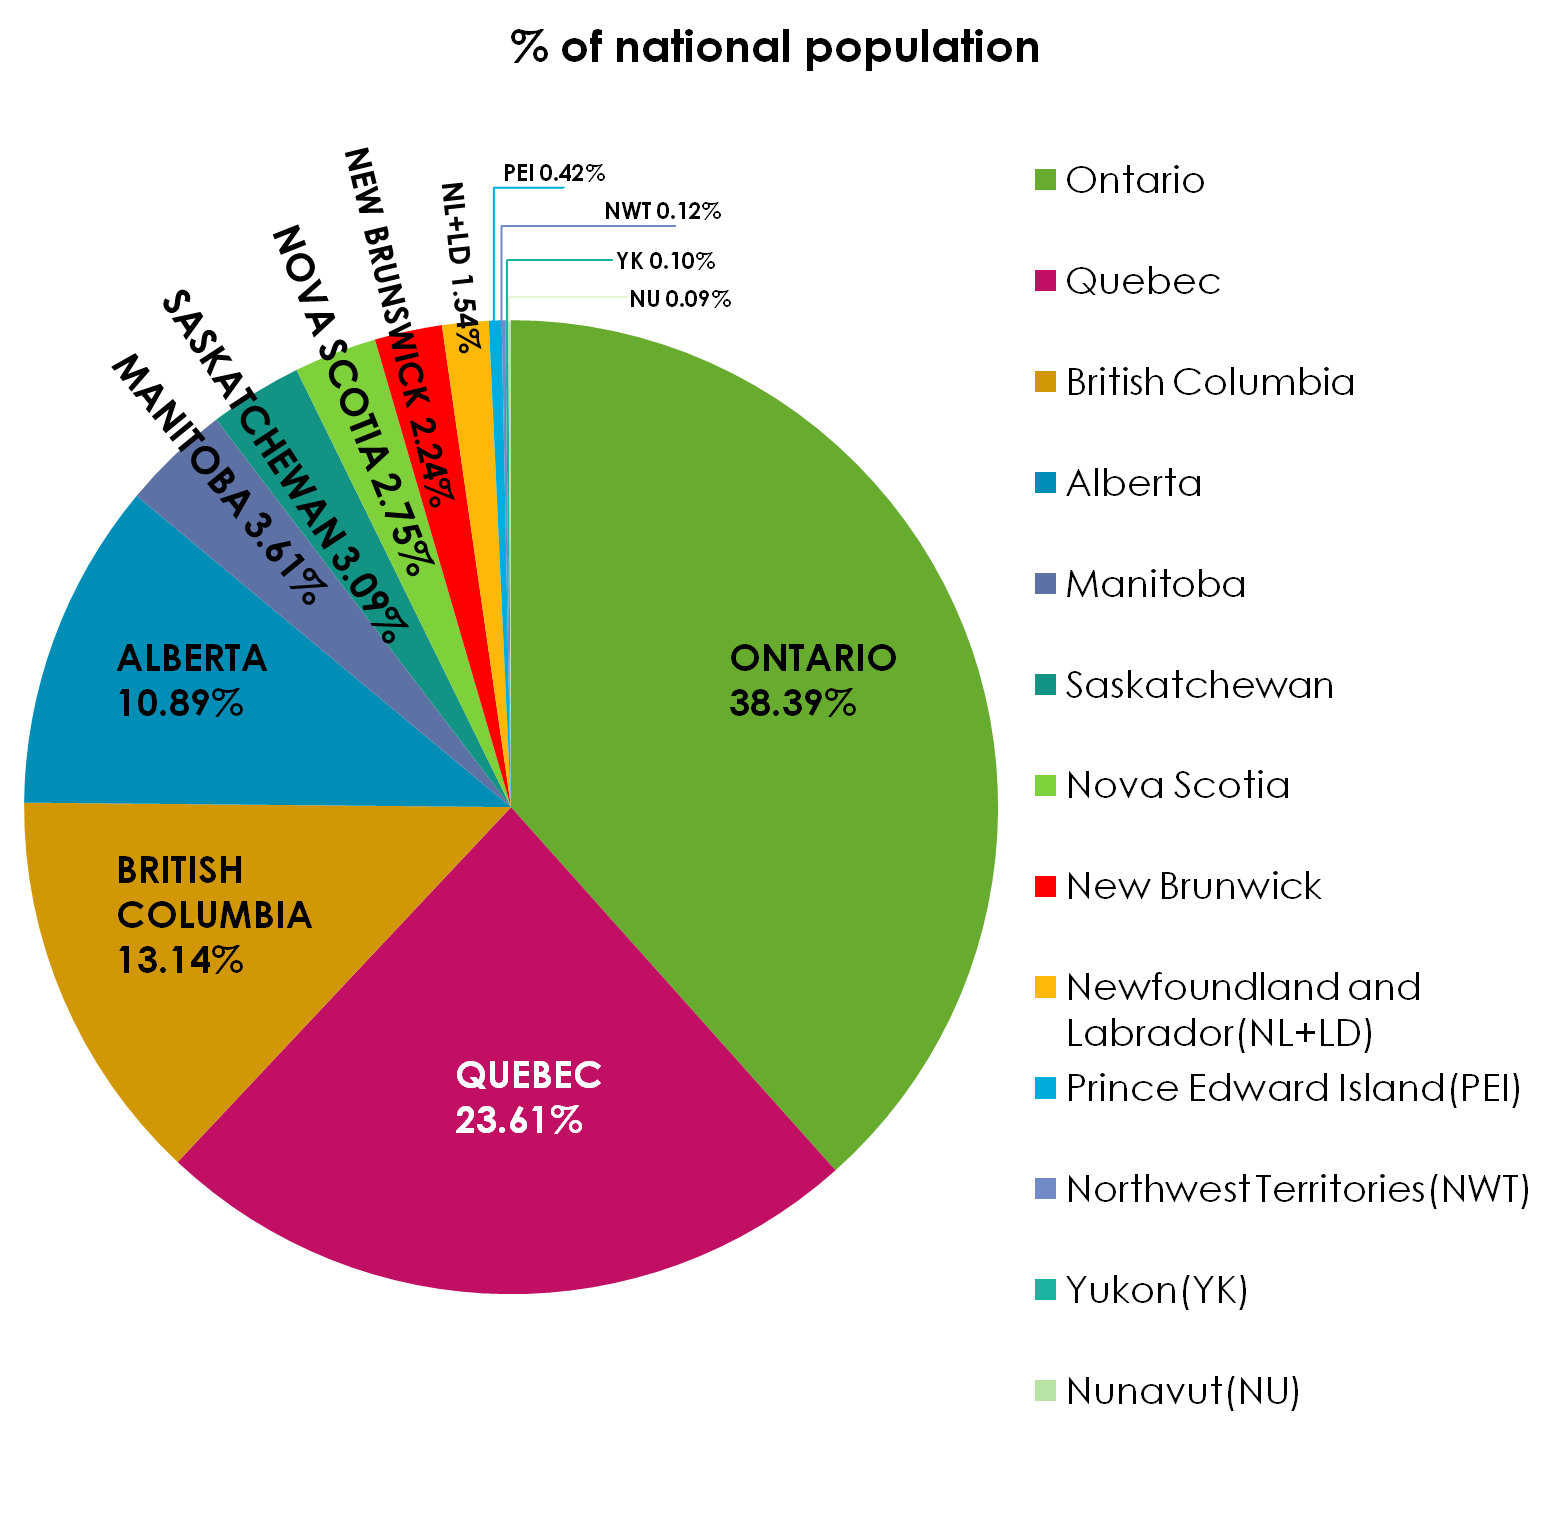
\includegraphics[width=\linewidth]{PopulationCanada.png}
\end{column}
\begin{column}{0.5\linewidth}
{\bf Bar graph}: the height of the bar
is proportional to the frequency\\
\medskip

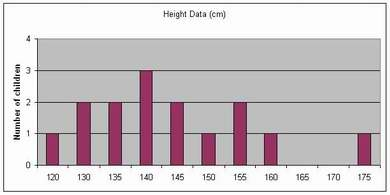
\includegraphics[width=\linewidth]{height.jpg}
\end{column}
\end{columns}

General rule: Use a bar graph whenever the data can be ordered, e.g. numbers.
For qualitative data, e.g. colors, a pie chart may be more appropriate.
\end{frame}

\begin{frame}
A {\bf histogram} displays quantitative data like a bar graph, but it allows
for unequal block lengths. 
\medskip

\begin{center}
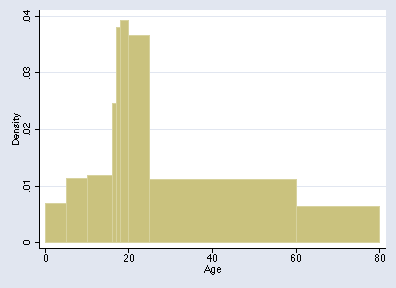
\includegraphics[height=0.4\textheight]{histogram}
\end{center}

Main principle: Area is proportional to frequency.\\
So the percentage falling into a block can be figured without
a vertical scale since the total area equals 100\%.\\
But it's helpful to have a vertical scale ({\sl density scale}).
Its unit is `\% per unit', so `\% per year' in above example.\\
\end{frame}

\begin{frame}
\begin{center}
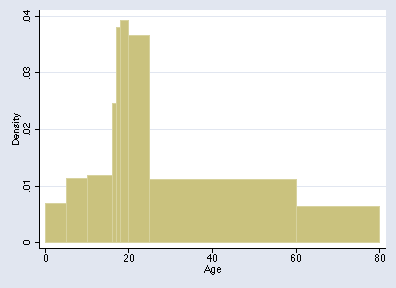
\includegraphics[height=0.4\textheight]{histogram}
\end{center}

The histogram gives two kinds of information about the data:\\
\smallskip

1. {\bf Density} (crowding): The height of the bar tells how many subjects are
for one unit on the horizontal scale. For example, the highest density is around age 19 as
$.04=4\%$ of all subjects have ages in the range 19--20 years. In contrast, only about $0.7\%$ of
subjects fall into each one year range for ages 60--80. 
\end{frame}

\begin{frame}
\begin{center}
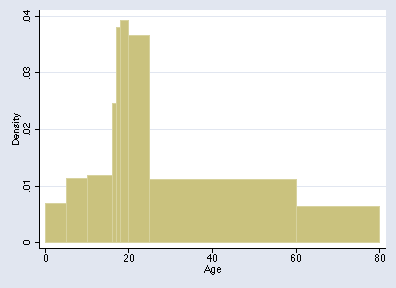
\includegraphics[height=0.4\textheight]{histogram}
\end{center}

The histogram gives two kinds of information about the data:\\
\smallskip

2. {\bf Percentages} (relative frequences): Those are given by\\
\begin{center}
 area = height x width.\\
\end{center}
For example, about $14\%$ of all subjects fall into the age range 60--80, because the
corresponding area is\\
 (20 years) x (0.7 \% per year)=14 \%. Alternatively, you can find
this answer by eyeballing that the area makes up roughly 1/7 of the total 
area of the histogram, so
roughly 1/7=14\% of all subjects fall in that range.
\end{frame}

\begin{frame}
The {\bf box plot} (or: box-and-whisker plot) is a more compact graphical
summary depicting 5 numbers: the minimum and maximum, and the 1st, 2nd
and 3rd quartiles. 
\medskip

\begin{center}
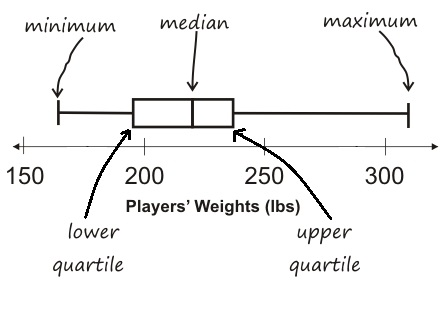
\includegraphics[height=0.5\textheight]{boxplot}
\end{center}

The box plot gives an indication of skewness in the data.
\end{frame}

\begin{frame}
The compact display of the box plot makes it well suited for 
comparing several data sets:
\medskip

\begin{center}
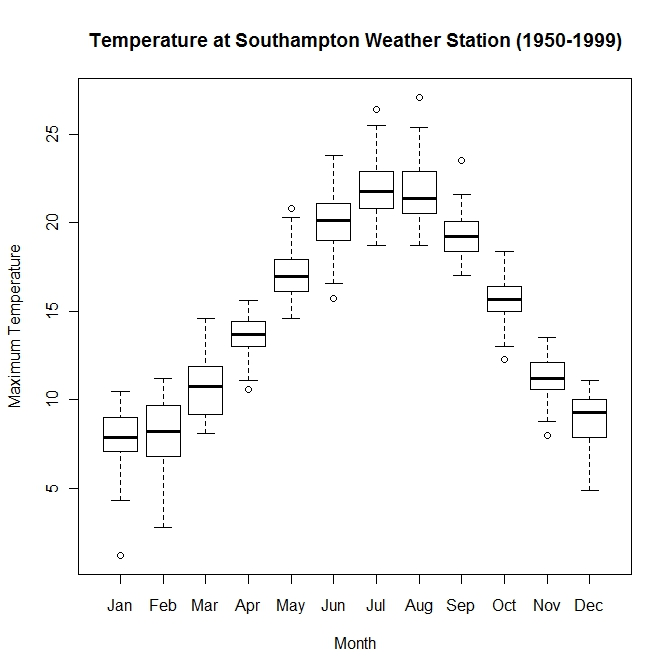
\includegraphics[height=0.6\textheight]{boxplotmultiple}
\end{center}

This is an example of the principle of `small multiples', 
which we will discuss later.
\end{frame}

\begin{frame}
For bivariate data, the standard display is the scatterplot. 
It visualizes association between the two variables.

\begin{center}
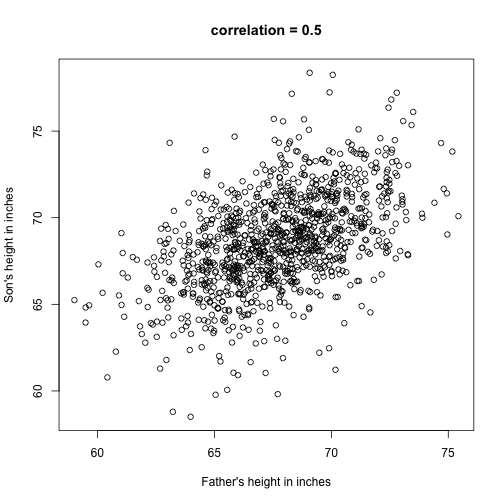
\includegraphics[height=0.7\textheight]{Galton}
\end{center}

\end{frame}

\begin{frame}
If there are many points then one needs to use shading to avoid big blobs:
\begin{center}
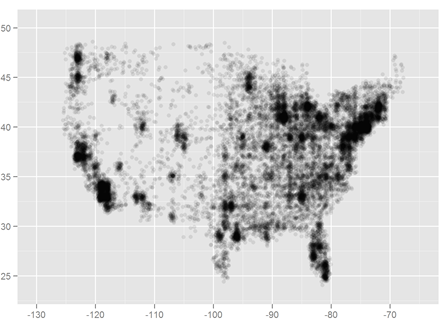
\includegraphics[height=0.5\textheight]{us}
\end{center}
Scatterplot of latitude and longitude of visitors to a web site.\\
Note how faint grid lines help to interpret the data.
\end{frame}

\begin{frame}
For more than 2 variables sometimes a useful visualization
obtains by using scatter + (size,color,\ldots)

\begin{center}
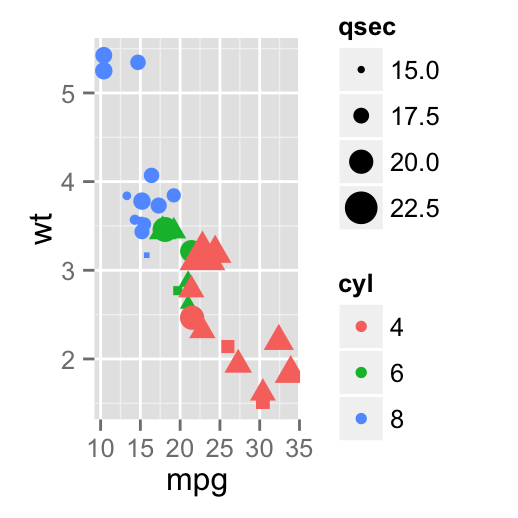
\includegraphics[height=0.7\textheight]{mtcars}
\end{center}

`mtcars' in R with ggplot
\end{frame}

\begin{frame}
An alternative is the scatter plot matrix:

\begin{center}
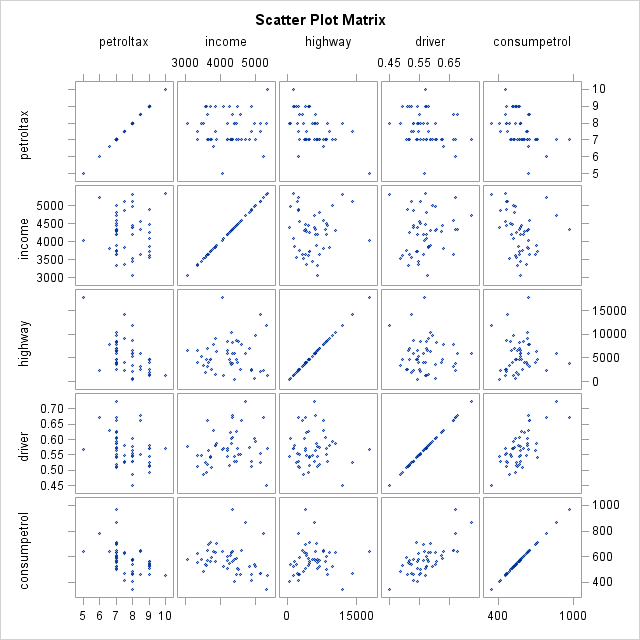
\includegraphics[height=0.8\textheight]{ScatterPlotMatrix}
\end{center}
\end{frame}

\begin{frame}
The principle of displaying {\sl small multiples} is well suited
for visualizing differences in objects or changes over time as the human
brain is good at processing small multiples.

\begin{center}
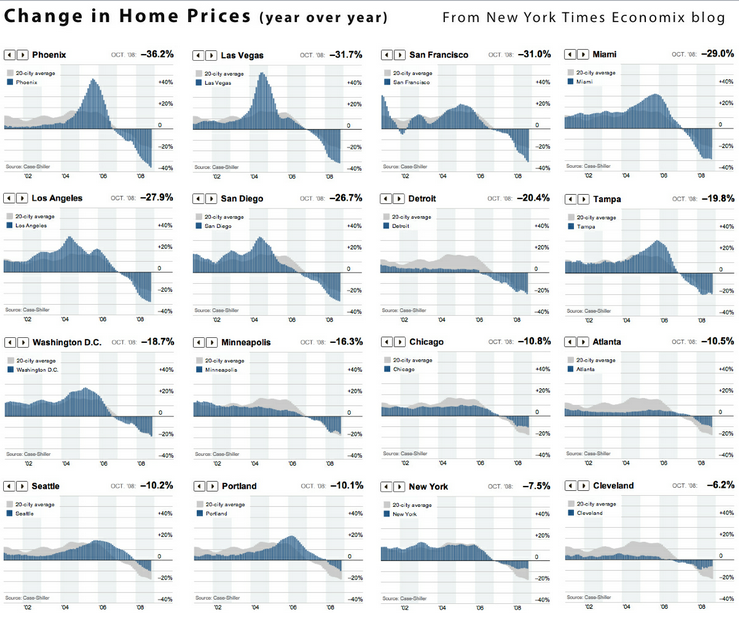
\includegraphics[height=0.7\textheight]{smallmultiples}
\end{center}
\end{frame}
 
\begin{frame}
\frametitle{Graphics software makes it tempting to produce
showy but poor visualizations}

\begin{center}
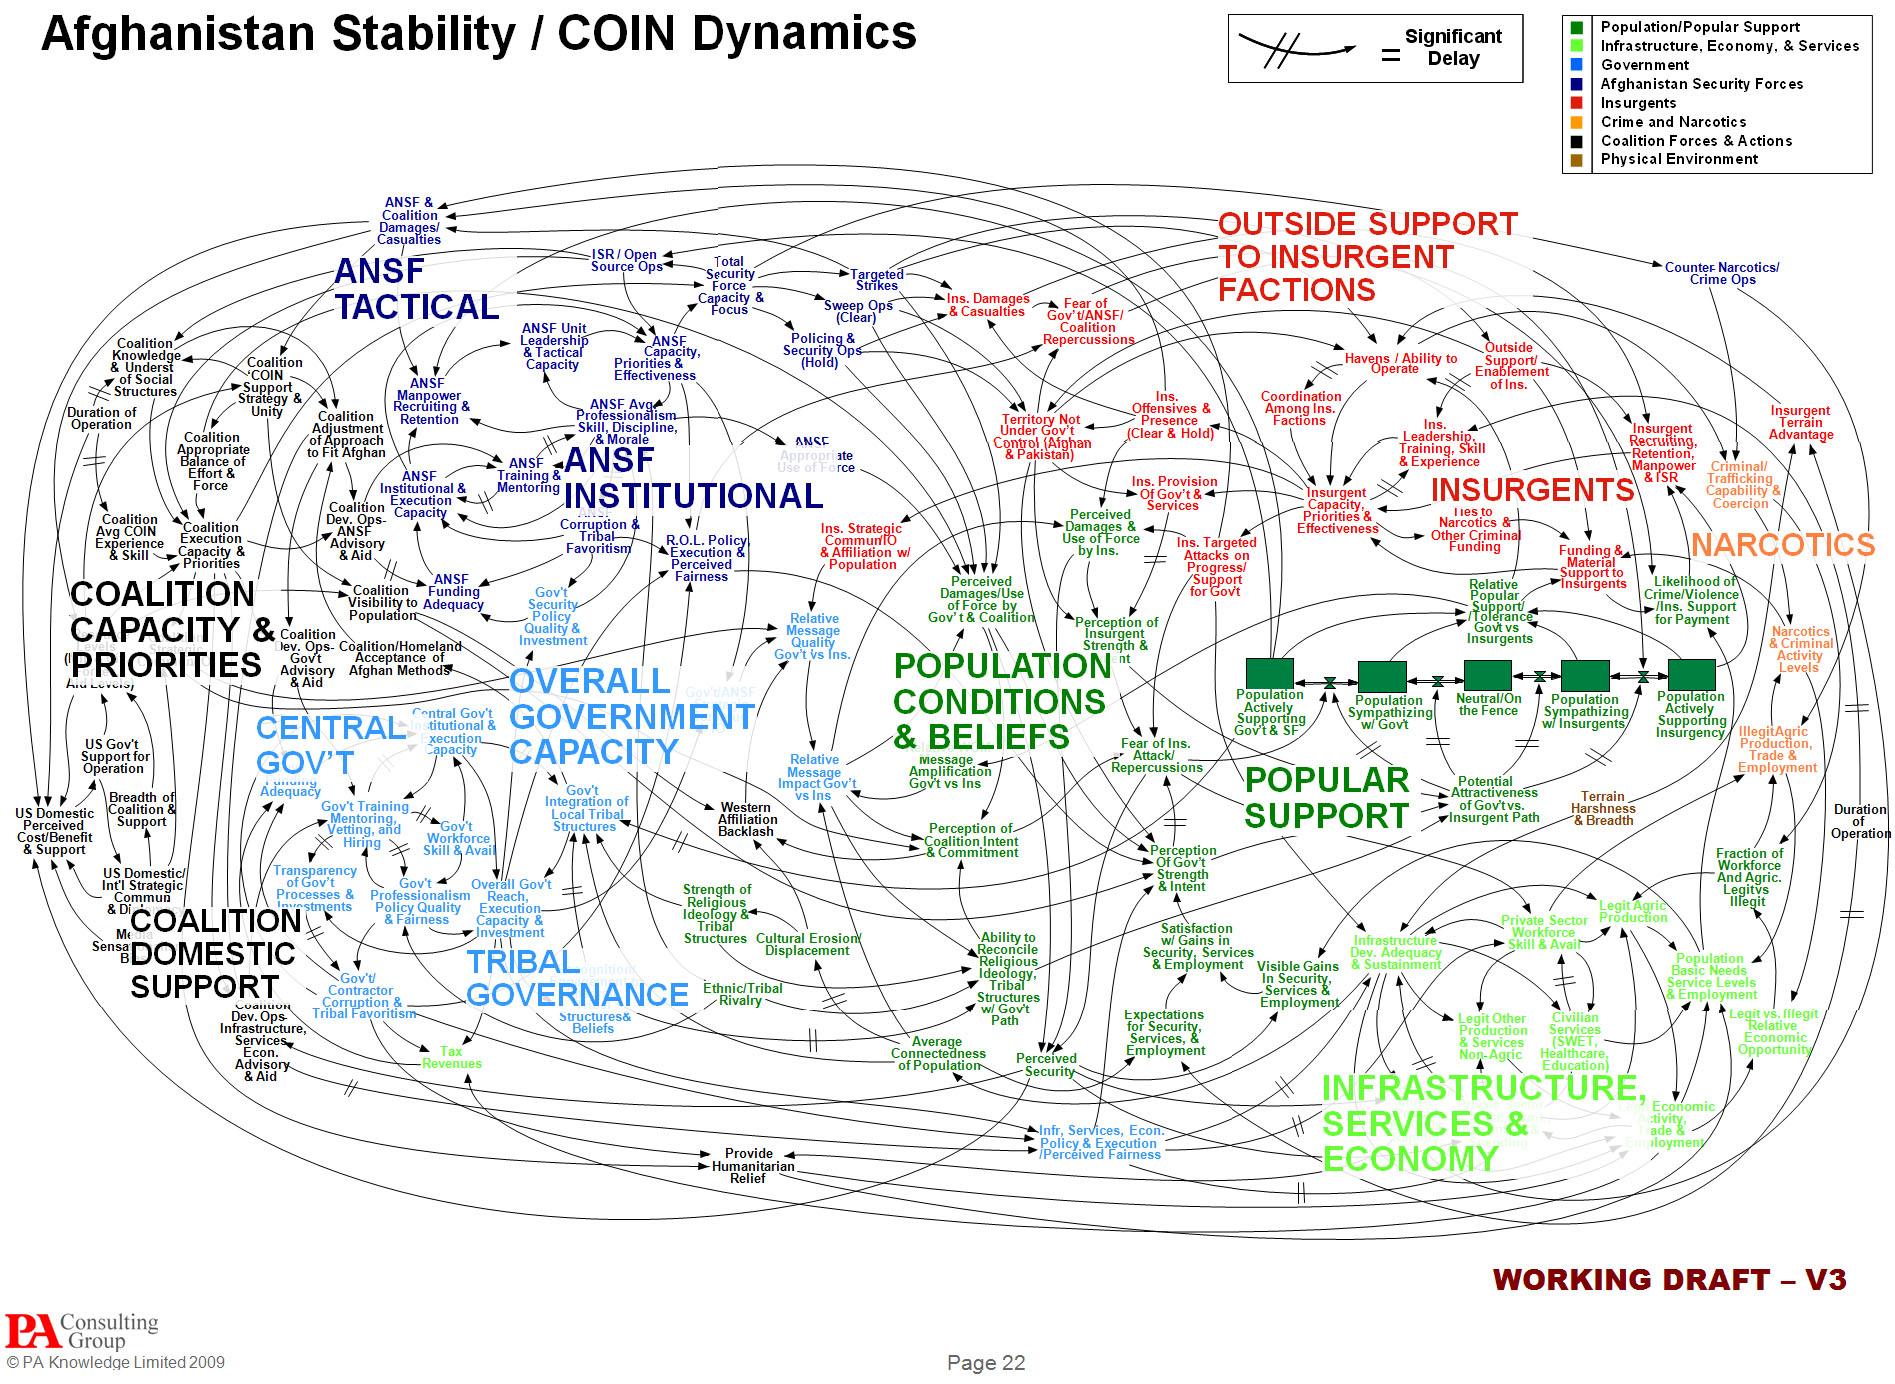
\includegraphics[height=0.6\textheight]{AfghanCoin}
\end{center}

from the New York Times (4/26/2010): We Have Met the Enemy and He
Is PowerPoint.
\end{frame}

\begin{frame}
\frametitle{Graphics software makes it tempting to produce
showy but poor visualizations}
\begin{center}
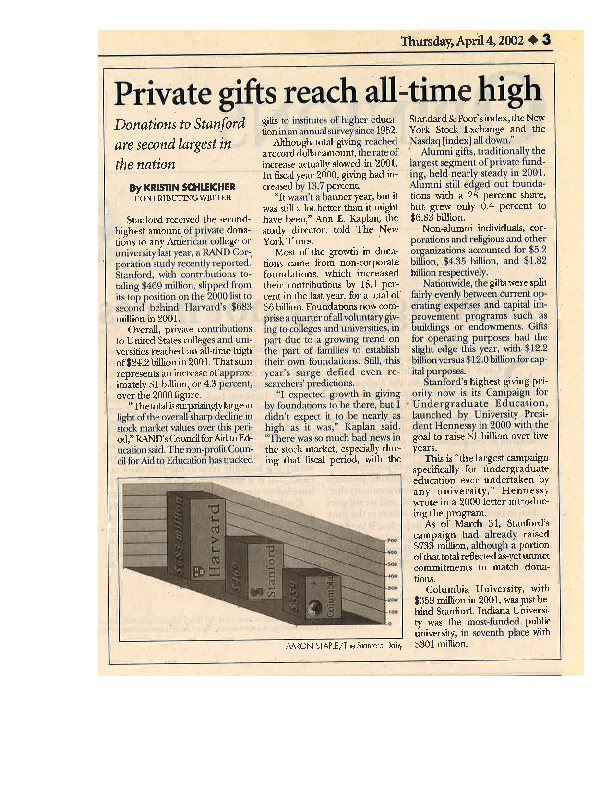
\includegraphics[height=0.8\textheight]{StanfordDailyGifts}
\end{center}
\end{frame}

\begin{frame}
\frametitle{What is good way to visualize data?}
There is a large number of ways to display data.\\
Which displays are good and why?
\medskip

Cleveland (who coined the name `Data Science' around the time you
were born) and McGill developed a simple taxonomy based on {\sl
graphical perception}: 
\medskip

They identified ten {\sl elementary perceptual
tasks} and then they did experiments to find out which tasks are easy or
difficult for the human brain. This provides a guideline for the
use of existing and the construction of new visualization techniques.
\end{frame}

\begin{frame}
\frametitle{The 10 elementary perceptual tasks}

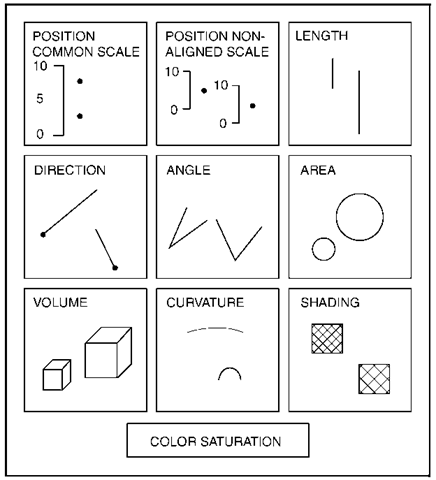
\includegraphics[height=0.8\textheight]{CMElemTasks}
\end{frame}

\begin{frame}
\frametitle{Examples of the elementary perceptual tasks}
Position on a common scale: bar graph\\
Angle: pie chart\\
Shading: {\sl statistical maps} display information as a function of
geographical location:

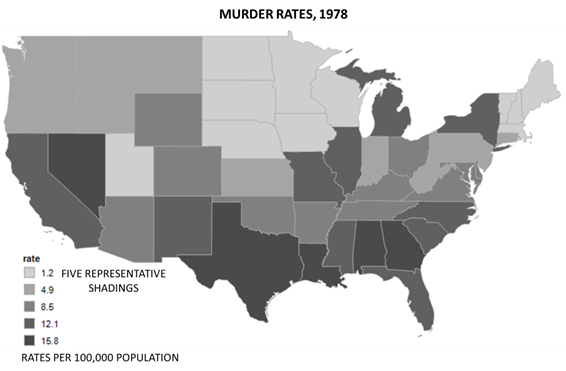
\includegraphics[height=0.6\textheight]{CMFig5}
\end{frame}

\begin{frame}
\frametitle{Ranking of the 10 elementary tasks}
\begin{columns}[T]
\begin{column}{0.5\linewidth}
\begin{enumerate}
\item Position along a common scale
\item Position along nonaligned scales
\item Length, direction, angle
\item Area
\item Volume, curvature
\item Shading, color saturation
\end{enumerate}
\end{column}
\begin{column}{0.5\linewidth}
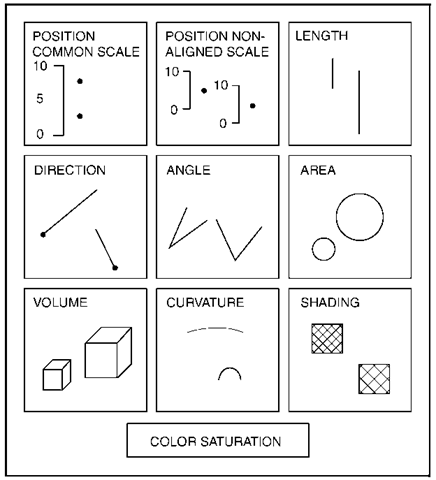
\includegraphics[height=0.6\textheight]{CMElemTasks}
\end{column}
\end{columns}
\end{frame}

\begin{frame}
For an illustration, note that `assessing length' is not ranked
near the top. This task comes up for {\sl curve-difference charts},
where the vertical difference between two curves has to be assessed:
\medskip

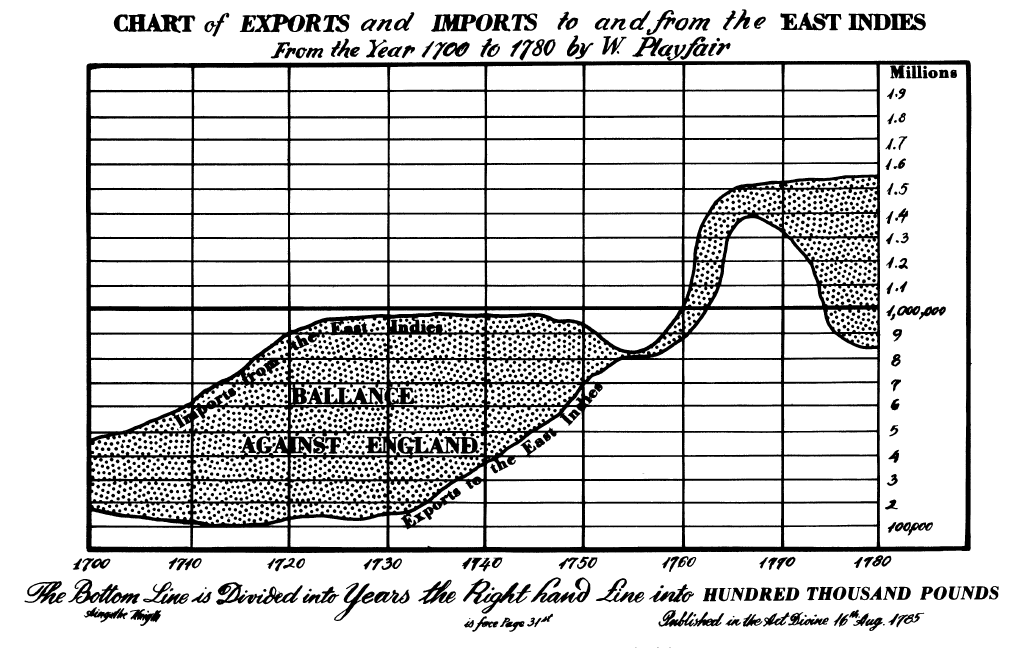
\includegraphics[height=0.6\textheight]{CMFig6}
\end{frame}

\begin{frame}
Assessing length is difficult for the eye-brain system:
\medskip

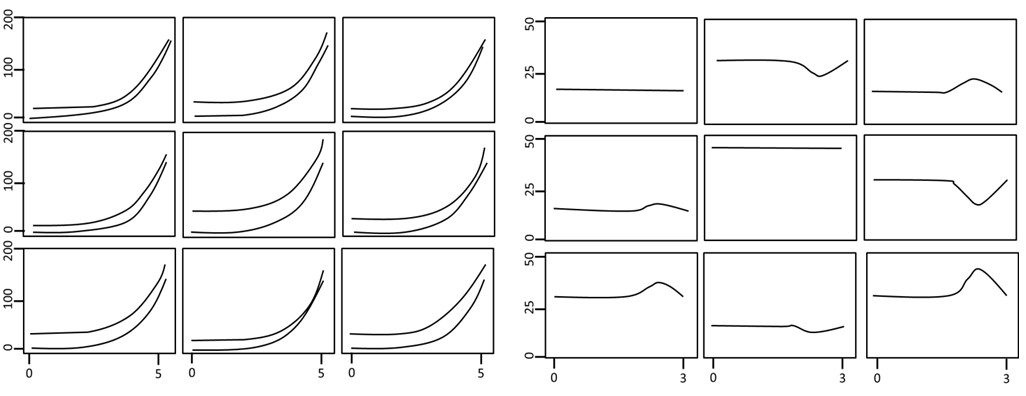
\includegraphics[width=\textwidth]{CMFig26}

The plots in the right panel show the differences between the pairs
of curves in the left panel.
\end{frame}

\begin{frame}
The next example illustrates why it is easier to judge position
on an nonaligned scale than to assess length:
\begin{columns}[T]
\begin{column}{0.5\linewidth}
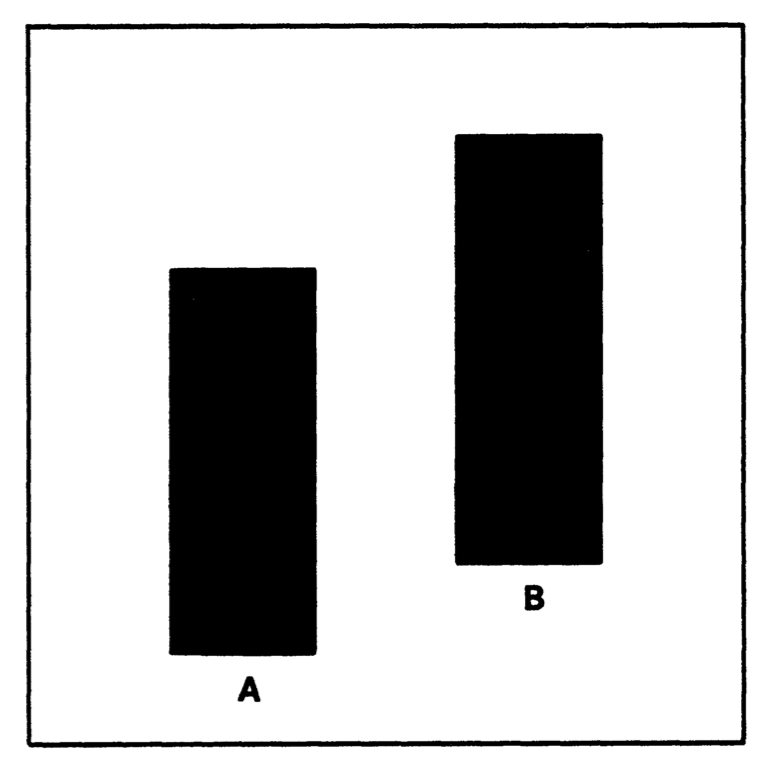
\includegraphics[height=0.6\textheight]{CMFig12a}
\end{column}
\begin{column}{0.5\linewidth}
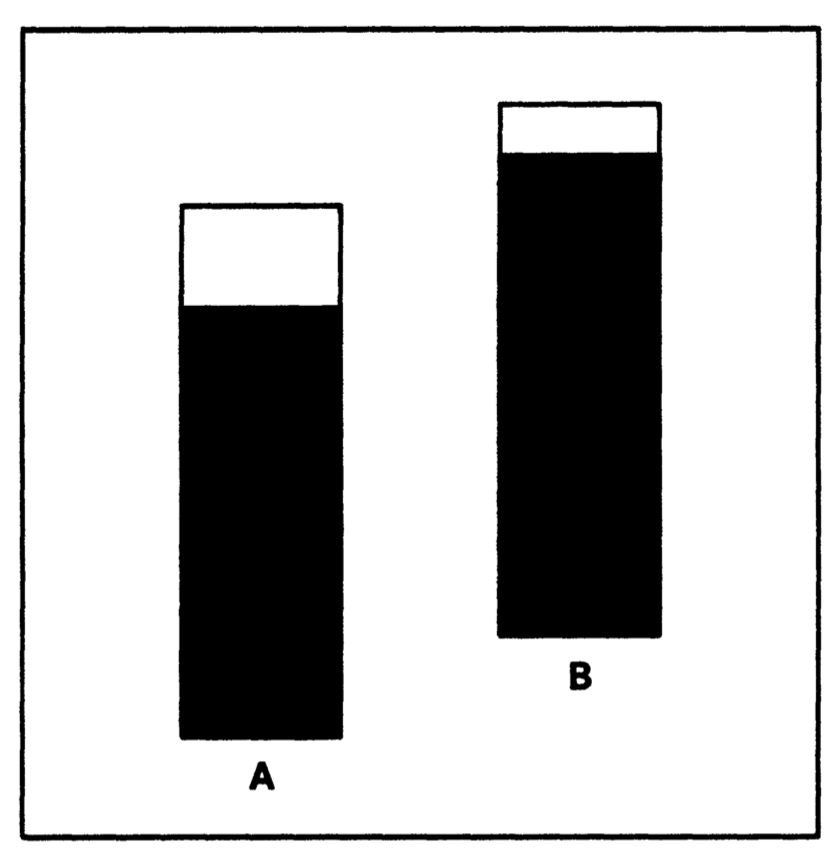
\includegraphics[height=0.6\textheight]{CMFig12b}
\end{column}
\end{columns}
This fact can also be derived from psychophysical theory:\\
It follows
from Weber's law that the difficulty in comparing lengths
depends on the ratio of the lengths, not their difference.\\
Using a bounding box helps as the ratio of the white bars is 
clearly different from 1, while that of the black bars isn't.
\end{frame}

\begin{frame}
This ordering of the elementary tasks leads to the following
important principle for choosing or developing methods for
visualization:
\medskip

Whenever possible, employ tasks that are ranked high on the list:
\medskip

\begin{enumerate}
\item Position along a common scale
\item Position along nonaligned scales
\item Length, direction, angle
\item Area
\item Volume, curvature
\item Shading, color saturation
\end{enumerate}
\end{frame}

\begin{frame}
For example, Cleveland McGill advocate replacing a pie chart with a bar graph
or a {\sl dot chart}, because perceiving position on a common scale
is easier than perceiving angles:
\medskip

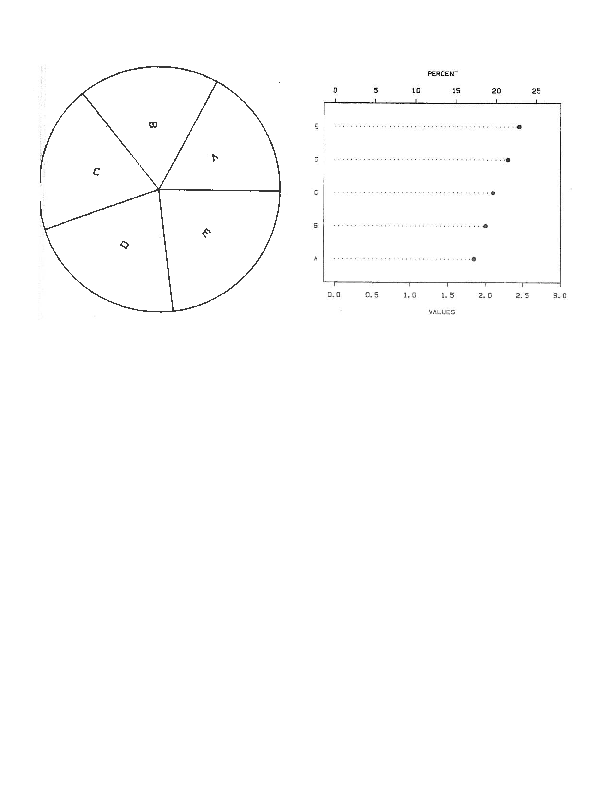
\includegraphics[width=\textwidth]{CMFig22}
\end{frame}

\begin{frame}
Positioning on a nonaligned scale in a divided bar chart can
be replaced by a dot chart with grouping, which uses positioning
on a common scale:
\medskip

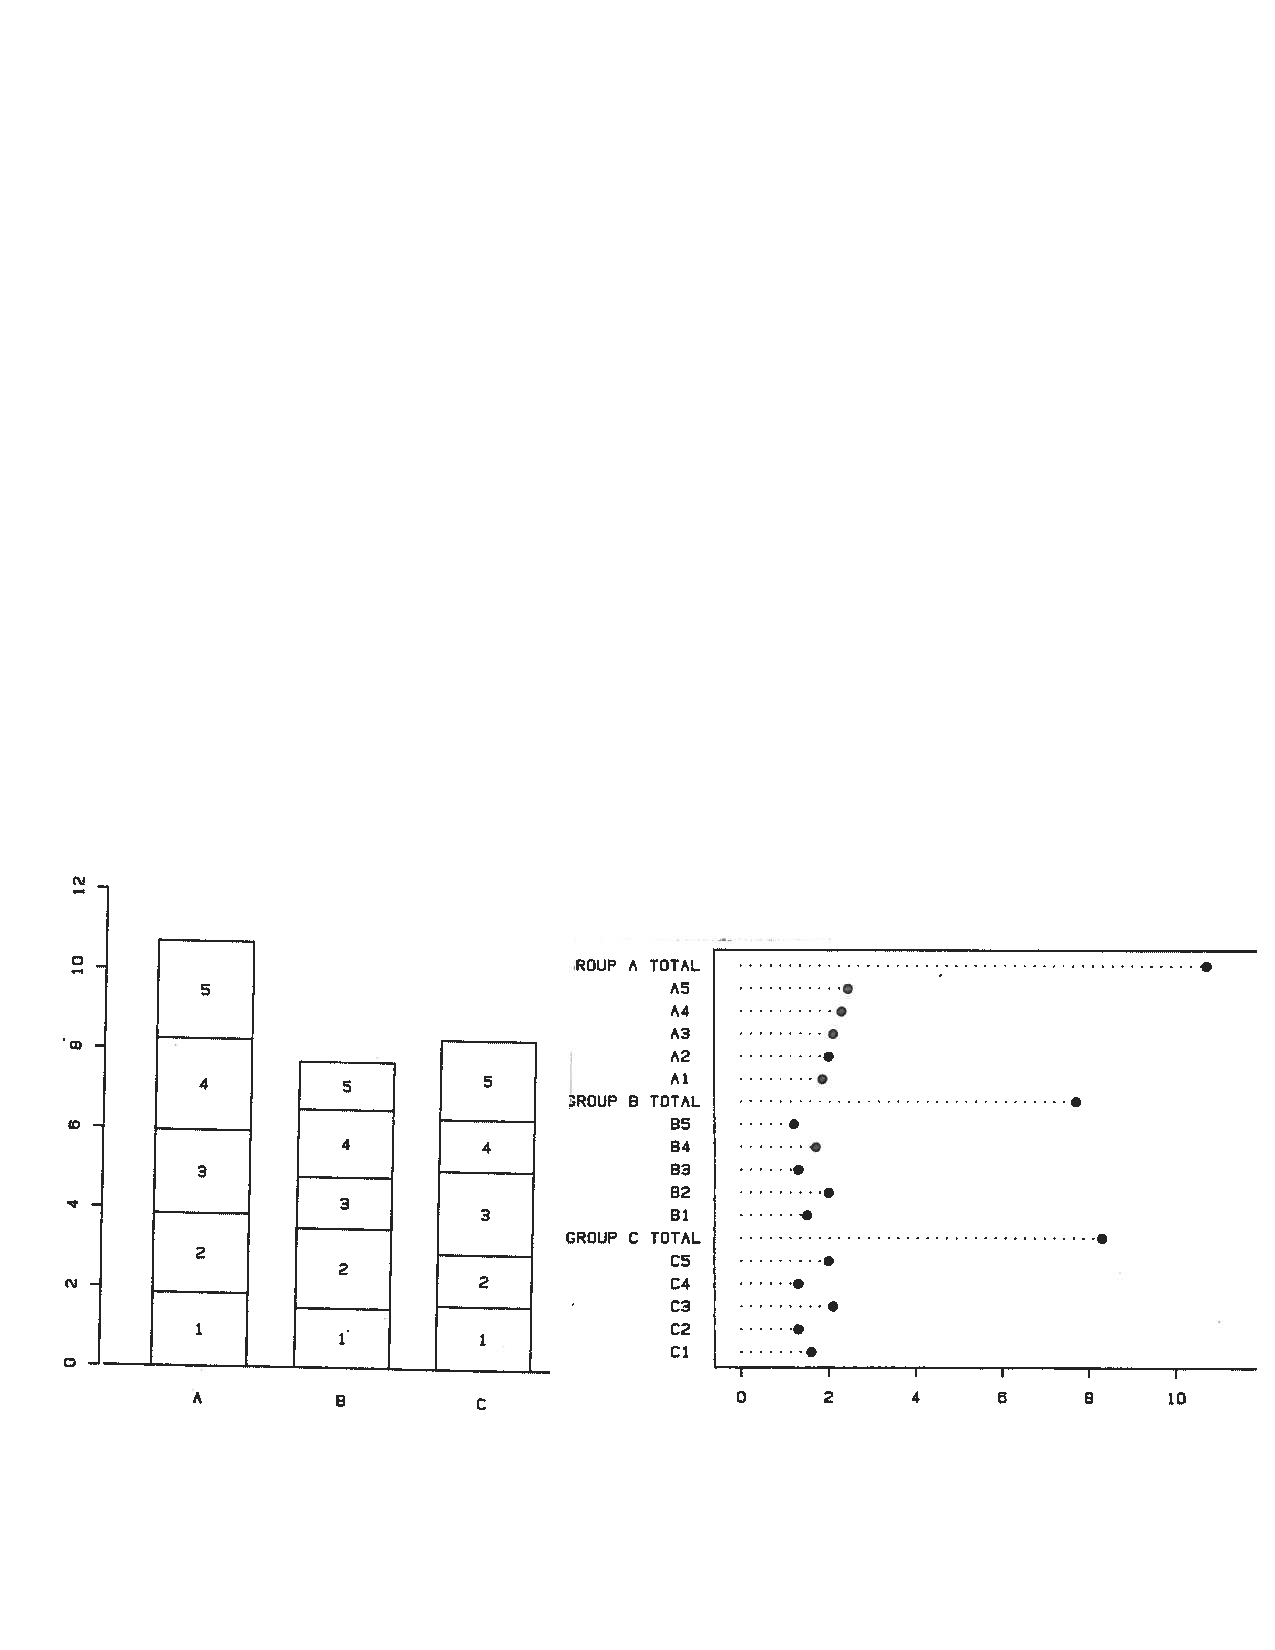
\includegraphics[height=0.6\textheight]{CMFig24}
\end{frame}

\begin{frame}
Judging length in a curve-difference chart can be replaced by
plotting the difference on a common scale:

\begin{center}
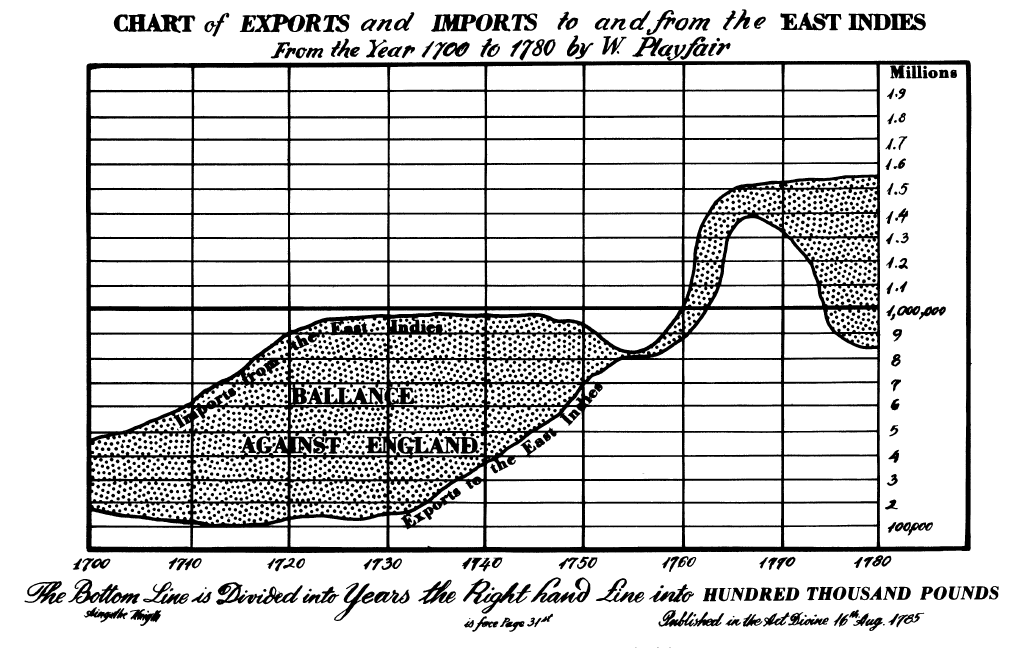
\includegraphics[height=0.4\textheight]{CMFig6}

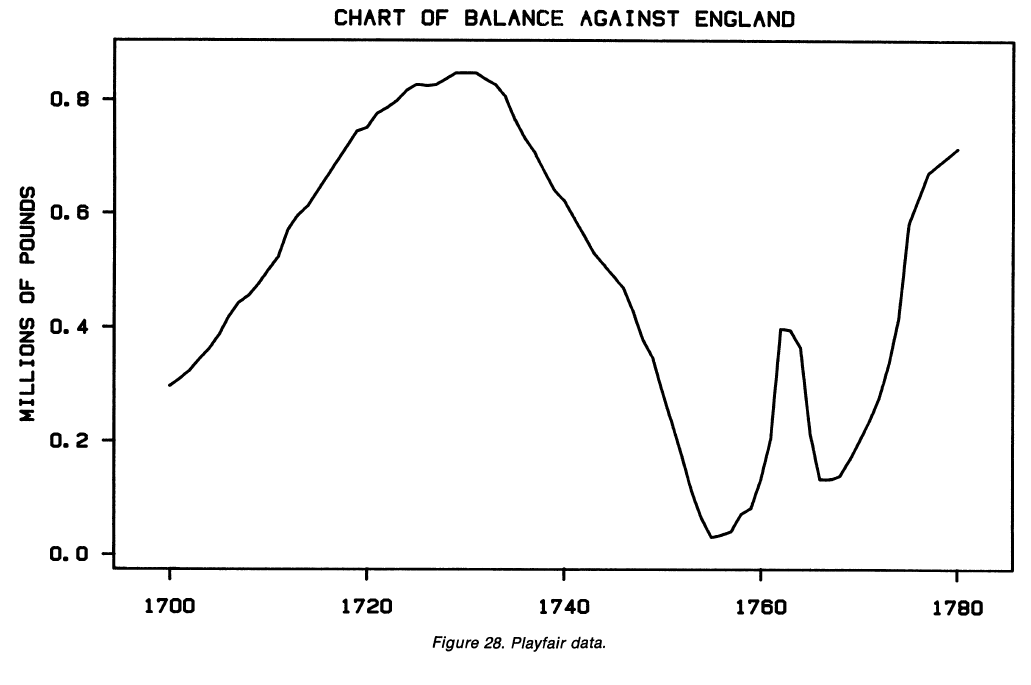
\includegraphics[height=0.4\textheight]{CMFig28}
\end{center}
\end{frame}

\begin{frame}
Shading can be replaced by positioning on a nonaligned scale:

\begin{center}
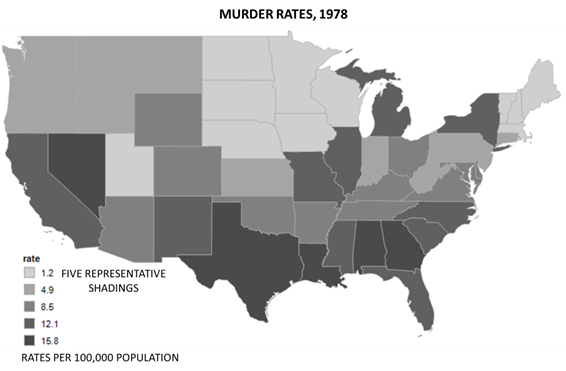
\includegraphics[height=0.4\textheight]{CMFig5}

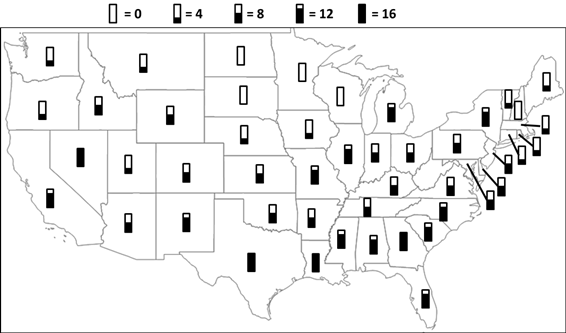
\includegraphics[height=0.4\textheight]{CMFig29}
\end{center}
\end{frame}

\begin{frame}
\frametitle{Some important design considerations}
\begin{itemize}
\item Use perceptually effective encodings per the above ranking\\
\item Visualize the facts and only the facts\\
\item Reduce overhead
\item Context is essential for graphical integrity
\end{itemize}
\end{frame}

\begin{frame}
\frametitle{Some important design considerations}
\begin{itemize}
\item Use perceptually effective encodings per the above ranking.\\
Note that color is ranked low and should be avoided. Some guidelines
for using color:\\
\begin{itemize}
\item Hue (color) is perceived as unordered and should only be used
to label qualitative data.\\
\item Value (brightness) is perceived as ordered and can be used to code
quantitative data if the range in values is small.
\end{itemize}

\begin{center}
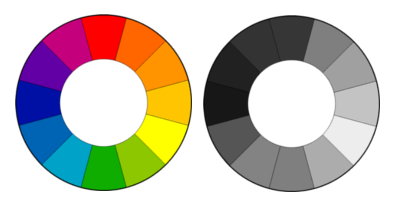
\includegraphics[height=0.4\textheight]{huevalue}
\end{center}

\end{itemize}
\end{frame}

\begin{frame}
\frametitle{Some important design considerations}
\begin{itemize}
\item Visualize the facts and only the facts\\
\begin{itemize}
\item Avoid chartjunk 

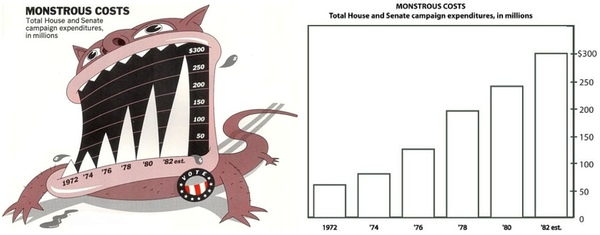
\includegraphics[height=0.35\textheight]{memory-monster}

\item `Connecting the dots' is often a borderline case: It suggests
there is more information displayed than there really is, but it helps
to visualize trends.

\begin{center}
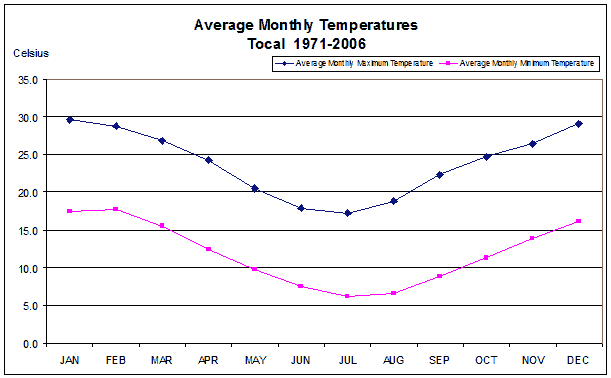
\includegraphics[height=0.3\textheight]{connectdots}
\end{center}

\end{itemize}
\end{itemize}
\end{frame}

\begin{frame}
\frametitle{Some important design considerations}
\begin{itemize}
\item Reduce overhead: 
\begin{itemize}
\item Avoid legend lookup if direct labeling works
\item Use faint grid lines: They provide more information if
needed and stay in the background otherwise.
\smallskip

\begin{center}
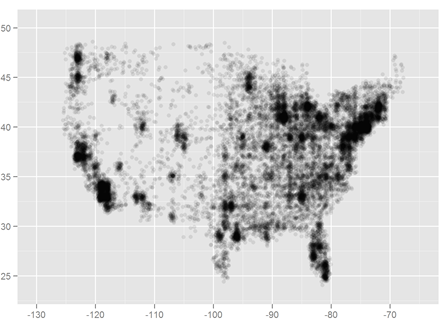
\includegraphics[height=0.4\textheight]{us}

Scatterplot of latitude and longitude of visitors to a web site.
\end{center}

\end{itemize}
\end{itemize}
\end{frame}

\begin{frame}
\frametitle{Some important design considerations}

\begin{center}
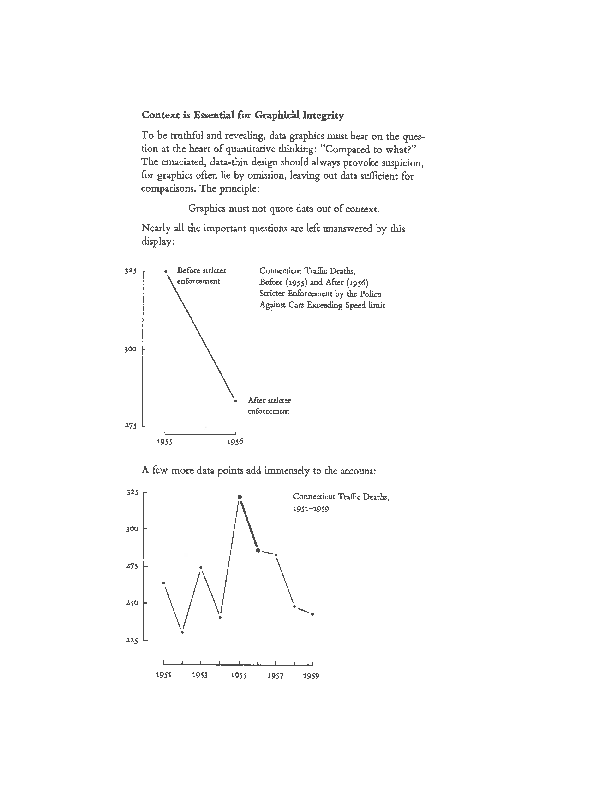
\includegraphics[height=0.9\textheight]{context1}
\end{center}

from Tufte: The Visual Display of Quantitative Information
\end{frame}

\begin{frame}
\begin{center}
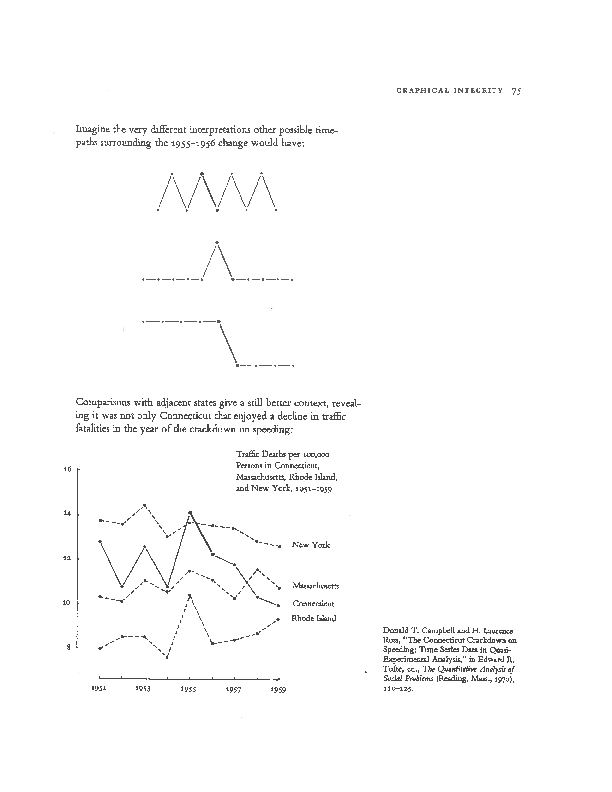
\includegraphics[height=0.9\textheight]{context2}
\end{center}


from Tufte: The Visual Display of Quantitative Information
\end{frame}

\end{document}
